\section{Ngoại lệ và xử lý ngoại lệ}
\label{exception}
\subsection{Ngoại lệ là gì? Các loại ngoại lệ trong Python}
Ngoại lệ (exception) là lỗi xuất hiện làm dừng chương trình đang thực thi. Trong Python hỗ trợ các lập trình viên xử lý ngoại lệ để duy trì hoạt động cho chương trình.\par
Các Exception sẵn có của Python thông thường được bắt nguồn từ BaseException. Trong khi đó các exception của lập trình viên nên thừa kế từ lớp Exception hoặc từ các lớp con của nó. 
\begin{figure}[h]
	\centering
	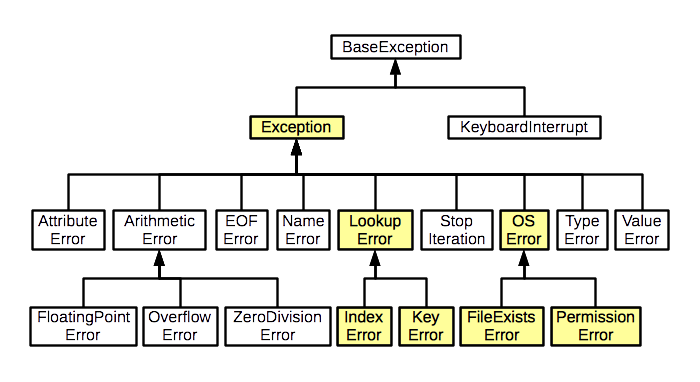
\includegraphics[width=0.7\linewidth]{img/exception}
	\caption{Sơ đồ mô tả các loại Exception trong Python}
\end{figure}
\newpage
\begin{table}[h]
	\centering
	\begin{tabular}{|l||p{12cm}|}
		\hline
		Tên ngoại lệ & Chú thích \\
		\hline
		\hline
		Exception & Đây là lớp cơ sở cho tất cả các exception, nó sẽ xuất hiện khi có bất cứ một lỗi nào xảy ra. \\
		\hline
		StopIteration & Xuất hiện khi phương thức next() của interator không trỏ đến một đối tượng nào.\\
		\hline
		SystemExit &	Xuất hiện khi dùng phương thức sys.exit().\\
		\hline
		ArithmeticError & Xuất hiện khi có lỗi tính toán giữa các số với nhau.\\
		\hline
		OverflowError &	Xuất hiện khi thực hiện tính toán và giá trị của nó vượt quá ngưỡng giới hạn cho phép của kiểu dữ liệu.\\
		\hline
		FloatingPointError &	Xuất hiện khi tính toán float thất bại.\\
		\hline
		ZeroDivisonError &	Xuất hiện khi thực hiện phép chia cho 0.\\
		\hline
		AssertionError &	Xuất hiện trong trường hợp lệnh assert thất bại.\\
		\hline
		AttributeError &	Xuất hiện khi không tồn tại thuộc tính này, hoặc thiếu tham số truyền vào nó.\\
		\hline
		EOFError &	Xuất hiện khi không có dữ liệu từ hàm input() hoặc cuối file.\\
		\hline
		ImportError &	Xuất hiện khi lệnh import thất bại.\\
		\hline
		KeyboardInterrupt &	Xuất hiện khi ngắt trình biên dịch.\\
		\hline
		LookupError &	Lớp cơ sở cho tất cả các lỗi về lookup.\\
		\hline
		IndexError &	Xuất hiện khi index không tồn tại trong list, string,...\\
		\hline
		KeyError &	Xuất hiện khi key không tồn tại trong dictionary.\\
		\hline
		NameError &	Xuất hiện khi một biến không tồn tại trong phạm vi bạn gọi nó.\\
		\hline
		EnvironmentError &	Xuất hiện khi có bất kỳ một lỗi nào ngoài phạm vi của Python.\\
		\hline
		IOError &	Xuất hiện khi xử dụng input/ output thất bại, hoặc  mở file không thành công.\\
		\hline
		OSError &	Xuất hiện khi có lỗi từ hệ điều hành.\\
		\hline
		SyntaxError &	Xuất hiện khi chương trình có lỗi cú pháp.\\
		\hline
		IndentationError &	Xuất hiện khi bạn thụt dòng không đúng.\\
		\hline
		SystemError &	Xuất hiện khi trình biên dịch có vấn đề nhưng mà nó lại không tự động exit.\\
		\hline
		SystemExit &	Xuất hiện khi trình biên dịch được thoát bởi sys.exit().\\
		\hline
		TypeError &	Xuất hiện khi thực thi toán tử hoặc hàm mà kiểu dữ liệu bị sai so với kiểu dữ liệu đã định nghĩa ban đầu.\\
		\hline
		ValueError &	Xuất hiện khi chúng ta build 1 function mà kiểu dữ liệu đúng nhưng khi chúng ta thiết lập ở tham số là khác so với khi truyền vào.\\
		\hline
		RuntimeError &	Xuất hiện khi lỗi được sinh ra không thuộc một danh mục nào.\\
		\hline
		NotImplementedError &	Xuất hiện khi một phương thức trừu tượng cần được thực hiện trong lớp kế thừa chứ không phải là lớp thực thi.\\
		\hline
		UnboundLocalError &	Xuất hiện khi chúng ta cố tình truy cập vào một biến trong hàm hoặc phương thức, nhưng không thiết lập giá trị cho nó.\\
		\hline
	\end{tabular}
	\caption{Các ngoại lệ trong Python}
\end{table}
\newpage
\textbf{Ví dụ:} Duyệt qua một list số nguyên, in ra giá trị nghịch đảo của từng phần tử trong list:\\
\rule{\linewidth}{0.2mm}\par
\begin{linenumbers}
	\texttt{list = [4, 5, 0, 7]}\par
	\texttt{\textcolor{red}{for} i \textcolor{red}{in} list:}\par
	\qquad\texttt{\textcolor{blue}{print}(1 / i)}\par
\end{linenumbers}
\rule{\linewidth}{0.2mm}\par
\noindent
\resetlinenumber
Kết quả cho ra ở Console:\\
\rule{\linewidth}{0.2mm}\par
\begin{linenumbers}
	\texttt{0.25}\par
	\texttt{0.2}\par
	\texttt{Traceback (most recent call last):}\par
	\texttt{File "Exception.py", line 3, in <module>}\par
	\qquad\texttt{print(1/i)}\par
	\texttt{ZeroDivisionError: division by zero}
\end{linenumbers}
\rule{\linewidth}{0.2mm}\par
\resetlinenumber
Khi duyệt đến phần tử \texttt{array[2] = 0}, việc tính toán giá trị $\frac{1}{i}$ gặp lỗi chia cho 0. Do đó, chương~trình dừng lại ngay lập tức và in lỗi ra ngoài Console, không tiếp tục duyệt các phần tử còn lại của list.
\newpage
\textbf{Ví dụ:} Duyệt qua một list chứa nhiều kiểu dữ liệu, in ra tổng giá trị các số trong list:\\
\rule{\linewidth}{0.2mm}\par
\begin{linenumbers}
	\texttt{list = [1, 2.3, 7.6, "Ex"]}\par
	\texttt{sum = 0.0}\par
	\texttt{\textcolor{red}{for} i \textcolor{red}{in} list:}\par
	\qquad\texttt{sum += i}\par
	\texttt{\textcolor{blue}{print}(sum)}\par
\end{linenumbers}
\rule{\linewidth}{0.2mm}\par
\noindent
\resetlinenumber
Kết quả cho ra ở Console:\\
\rule{\linewidth}{0.2mm}\par
\begin{linenumbers}
	\texttt{Traceback (most recent call last):}\par
	\texttt{File "Exception.py", line 4, in <module>}\par
	\qquad\texttt{sum += i}\par
	\texttt{TypeError: unsupported operand type(s) for +=: 'float' and 'str'}
\end{linenumbers}
\rule{\linewidth}{0.2mm}\par
Khi duyệt đến phần tử \texttt{"Ex"}, Python không thể chuyển kiểu dữ liệu chuỗi sang kiểu số và cộng vào biến \texttt{sum}, từ đó xảy ra lỗi \texttt{TypeError}.
\resetlinenumber
\newpage
\subsection{Xử lý ngoại lệ với try - except - finally}
Ta có thể xử lý ngoại lệ bằng cách đặt phần code có khả năng xảy ra lỗi vào trong câu lệnh \texttt{try - except}. Lập trình viên có thể in các mô tả về ngoại lệ xảy ra trong đoạn code ra màn hình, hoặc có thể bỏ qua chúng.\par
Cấu trúc câu lệnh try - catch - finally:\par
\rule{\linewidth}{0.2mm}\par
\texttt{try:}\par
\qquad\texttt{\# code}\par
\texttt{except <exception\_name> as <variable\_name>:}\par
\qquad\texttt{\# handle code}\par
\texttt{[finally:}\par
\qquad\texttt{\# code]}\par
\rule{\linewidth}{0.2mm}\par
Cách thức hoạt động của try - catch - finally diễn ra như sau: Khi các câu lệnh trong try được phát hiện xảy ra ngoại lệ, chương trình sẽ chuyển xuống phần except và thực hiện các câu lệnh xử lý ngoại lệ trong nó. Sau khi xử lý xong ngoại lệ, tiếp tục thực hiện các câu lệnh trong finally (nếu có). Trường hợp trong try không có ngoại lệ, chương trình vẫn thực hiện các câu lệnh trong finally.\par
Khác với Java, lập trình viên có thể khai báo nhiều ngoại lệ có thể xảy ra trong chương trình mà không cần phải tuân thủ quy tắc từ cụ thể đến chung nhất. Python sẽ tự tìm kiếm một exception phù hợp trong các exception mà lập trình viên đã khai báo mà không quan tâm đến các ngoại lệ còn lại. Thứ tự xét các exception là từ trên xuống.
\newpage
\textbf{Ví dụ:} In các giá trị căn bậc 2 của từng phần tử trong một list, bỏ qua các giá trị âm:\\
\rule{\linewidth}{0.2mm}\par
\begin{linenumbers}
	\texttt{\textcolor{red}{from} math \textcolor{red}{import} sqrt}\par
	\medskip
	\texttt{list = [4, 16, -7, 25]}\par
	\texttt{\textcolor{red}{for} i \textcolor{red}{in} list:}\par
	\qquad\texttt{\textcolor{red}{try:}}\par
	\qquad\qquad\texttt{\textcolor{blue}{print}(sqrt(i))}\par
	\qquad\texttt{\textcolor{red}{except} Exception \textcolor{red}{as} e:}\par
	\qquad\qquad\texttt{\textcolor{red}{pass} \# skip if it's a negative number}\par
	\qquad\texttt{\textcolor{red}{finally}:}\par
	\qquad\qquad\texttt{\textcolor{blue}{print}("Done!")}\par
\end{linenumbers}
\rule{\linewidth}{0.2mm}\par
\noindent
\resetlinenumber
Kết quả cho ra ở Console:\\
\rule{\linewidth}{0.2mm}\par
\begin{linenumbers}
	\texttt{2.0}\par
	\texttt{Done!}\par
	\texttt{4.0}\par
	\texttt{Done!}\par
	\texttt{Done!}\par
	\texttt{5.0}\par
	\texttt{Done!}\par
\end{linenumbers}
\rule{\linewidth}{0.2mm}\par
\resetlinenumber
Khi xét đến phần tử -7, do không thể lấy căn bậc 2 của một số âm nên chương trình xét đoạn lệnh trong phần \texttt{except}. Từ khoá \texttt{pass} không thực hiện câu lệnh nào cả, chương trình chạy đến phần \texttt{finally}, in dòng chữ \texttt{"Done!"} ra ngoài màn hình rồi tiếp tục xét các giá trị khác trong list.
\newpage
\textbf{Ví dụ:} Duyệt và in ra các phần tử trong một list bằng chỉ số:\\
\rule{\linewidth}{0.2mm}\par
\begin{linenumbers}
	\texttt{ls = [1, 2, 0.2, 3]}\par
	\texttt{\textcolor{red}{for} i \textcolor{red}{in} range(len(ls) + 1):}\par
	\qquad\texttt{\textcolor{red}{try:}}\par
	\qquad\qquad\texttt{\textcolor{blue}{print}(ls[i])}\par
	\qquad\texttt{\textcolor{red}{except} ZeroDivisionError \textcolor{red}{as} e:}\par
	\qquad\qquad\texttt{\textcolor{blue}{print}(e)}\par
	\qquad\texttt{\textcolor{red}{except} LookupError \textcolor{red}{as} ex:}\par
	\qquad\qquad\texttt{\textcolor{blue}{print}(ex.\_\_doc\_\_)  \# output: Sequence index out of range.}\par
	\qquad\texttt{\textcolor{red}{except} IndexError \textcolor{red}{as} exc:}\par
	\qquad\qquad\texttt{\textcolor{blue}{print}(ex)  \# output: list index out of range.}\par
\end{linenumbers}
\rule{\linewidth}{0.2mm}\par
\noindent
\resetlinenumber
Kết quả cho ra ở Console:\\
\rule{\linewidth}{0.2mm}\par
\begin{linenumbers}
	\texttt{1}\par
	\texttt{2}\par
	\texttt{0.2}\par
	\texttt{3}\par
	\texttt{Sequence index out of range.}\par
\end{linenumbers}
\rule{\linewidth}{0.2mm}\par
\resetlinenumber
Do chỉ có 4 phần tử trong list \texttt{ls} nên các phần tử trong list được đánh số từ 0 đến 3. Hàm \texttt{range(len(ls)~+~1)} trả về một mảng số nguyên \texttt{[0, 1, 2, 3, 4]}. Khi duyệt đến phần tử có chỉ số 4 trong list, chương trình phát sinh ra lỗi và tìm đến exception phù hợp đầu tiên mà người lập trình đã khai báo là \texttt{LookupError} rồi thực hiện câu lệnh \texttt{print(ex.\_\_doc\_\_)}, bỏ qua exception \texttt{IndexError} mặc dù ngoại lệ này là cụ thể nhất cho lỗi phát sinh.
\newpage
\subsection{Ngoại lệ do người dùng tự định nghĩa}
Ngoài các ngoại lệ đã mô tả ở phần trên, lập trình viên có thể tự định nghĩa một ngoại lệ riêng sao cho phù hợp với từng chương trình cụ thể bằng từ khoá \texttt{raise}.\par
\textbf{Ví dụ:} Chương trình tính tiền thuê phòng khách sạn, mỗi giờ là \$5, số giờ không được dưới 1 và trên 12.:\\
\rule{\linewidth}{0.2mm}\par
\begin{linenumbers}
	\texttt{hour = [1, 5, 7, 0.5, 11]}\par
	\texttt{\textcolor{red}{for} i \textcolor{red}{in} hour:}\par
	\qquad\texttt{\textcolor{red}{if} i < 1 \textcolor{red}{or} i > 12:}\par
	\qquad\qquad\texttt{\textcolor{red}{raise} Exception("Hour must be greater than 1 and less than 12")}\par
	\qquad\texttt{\textcolor{blue}{print}("Price: \%d\$" \% (i * 5))}\par
\end{linenumbers}
\rule{\linewidth}{0.2mm}\par
\noindent
\resetlinenumber
Kết quả cho ra ở Console:\\
\rule{\linewidth}{0.2mm}\par
\begin{linenumbers}
	\texttt{Traceback (most recent call last):}\par
	\texttt{File "Exception.py", line 4, in <module>}\par
	\qquad\texttt{raise Exception("Hour must be greater than 1 and less than 12")}\par
	\texttt{Exception: Hour must be greater than 1 and less than 12}\par
	\texttt{Price: 5\$}\par
	\texttt{Price: 25\$}\par
	\texttt{Price: 35\$}\par
\end{linenumbers}
\rule{\linewidth}{0.2mm}\par
\resetlinenumber